\documentclass{beamer}

% Top-aligning columns within a top-aligned frame
% https://tex.stackexchange.com/questions/16447/beamer-top-aligning-columns-within-a-top-aligned-frame
\makeatletter
\newenvironment{myitemize}{%
   \setlength{\topsep}{0pt}
   \setlength{\partopsep}{0pt}
   \renewcommand*{\@listi}{\leftmargin\leftmargini \parsep\z@ \topsep\z@ \itemsep\z@}
   \let\@listI\@listi
   \itemize
}{\enditemize}
\makeatother  

\usepackage[USenglish]{babel}
\usepackage[utf8]{inputenc}
\usepackage{amssymb, amsmath}
\usepackage{bm}
\usepackage{color}
\usepackage{tikz}
\usepackage{url}

\definecolor{links}{HTML}{2A1B81}
\hypersetup{colorlinks,linkcolor=,urlcolor=links}

\usetheme{Boadilla}

\bibliographystyle{apalike}
% make bibliography entries smaller
%\renewcommand\bibfont{\scriptsize}
% Now get rid of all the colours
\setbeamercolor*{bibliography entry title}{fg=black}
\setbeamercolor*{bibliography entry author}{fg=black}
\setbeamercolor*{bibliography entry location}{fg=black}
\setbeamercolor*{bibliography entry note}{fg=black}

\newcommand{\lnorm}[1]{\left\lVert#1\right\rVert^2}
\newcommand{\norm}[1]{\left\lVert#1\right\rVert}

% and kill the abominable icon
\setbeamertemplate{bibliography item}{}

\begin{document}
\title[BigBird]{RandAugment: Practical automated data augmentation with a reduced search space}  
\author{Radek Bartyzal}
\date{22. 9. 2020} 
\institute{GLAMI AI}

\frame{\titlepage} 

%--------- END Frame 12 -------------
\begin{frame}{Motivation}

Training data augmentation = good.
\vfill
How to make it better?

\begin{itemize}
\item tailor the augmentations to your net + dataset
\item $\implies$ training the augmentation transformation 
\end{itemize}

\end{frame}
%--------- END Frame 12 -------------
\begin{frame}{Previous works}

\textbf{AutoAugment} \cite{cit:auto}
\begin{itemize}
\item 16 image transformation functions: f(image, magnitude)
\item each has 2 parameters:
\begin{itemize}
\item prob of applying the transformation (discretized 11 values)
\item magnitude of the transformation (discretized 10 values)
\end{itemize}
\item goal = find 5 transformations with proper params
\item use Reinforcement Learning (RL) to find them
\item RL reward = validation accuracy on a proxy task
\item proxy task = smaller net + subset of train dataset
\item cca 15000 policies (solutions) were sampled during training
\end{itemize}
\end{frame}
%--------- END Frame 12 -------------
\begin{frame}{RandAugment}

\begin{itemize}
\item 14 image transformation functions: f(image, magnitude)
\item selects all image transformations with
equal probability
\item only 2 params:
\begin{itemize}
\item[N:] number of randomly selected transformations
\item[M:] magnitude of all transformations
\end{itemize}
\item $\implies$ can be used as hyper-params during full training
\item $\implies$ no proxy task, directly optimize for the final net
\end{itemize}


\end{frame}
%--------- END Frame 12 -------------
\begin{frame}{RandAugment code}

\begin{figure}[h]
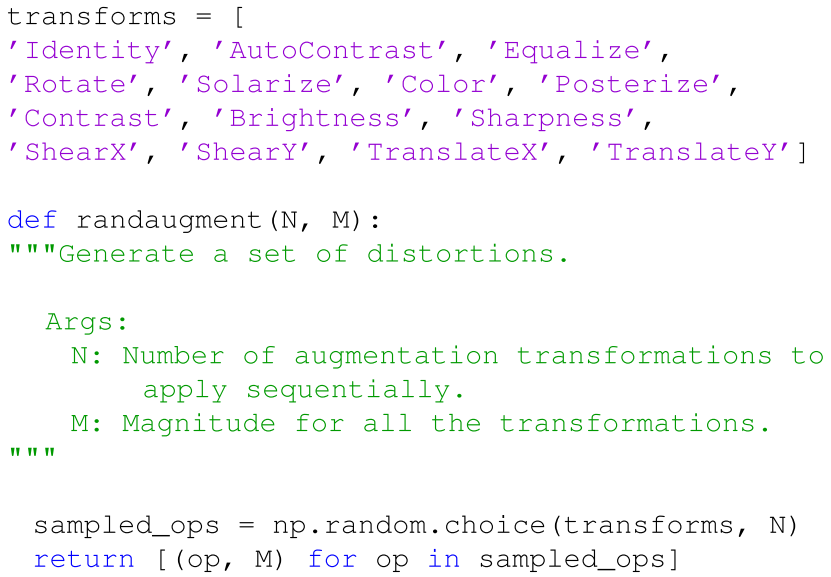
\includegraphics[width=0.8\textwidth]{img/code}
\caption{Only 2 params: $N$ and $M$.}
\end{figure}

\end{frame}
%--------- END Frame 12 -------------
\begin{frame}{RandAugment: example of augmented images}

\begin{figure}[h]
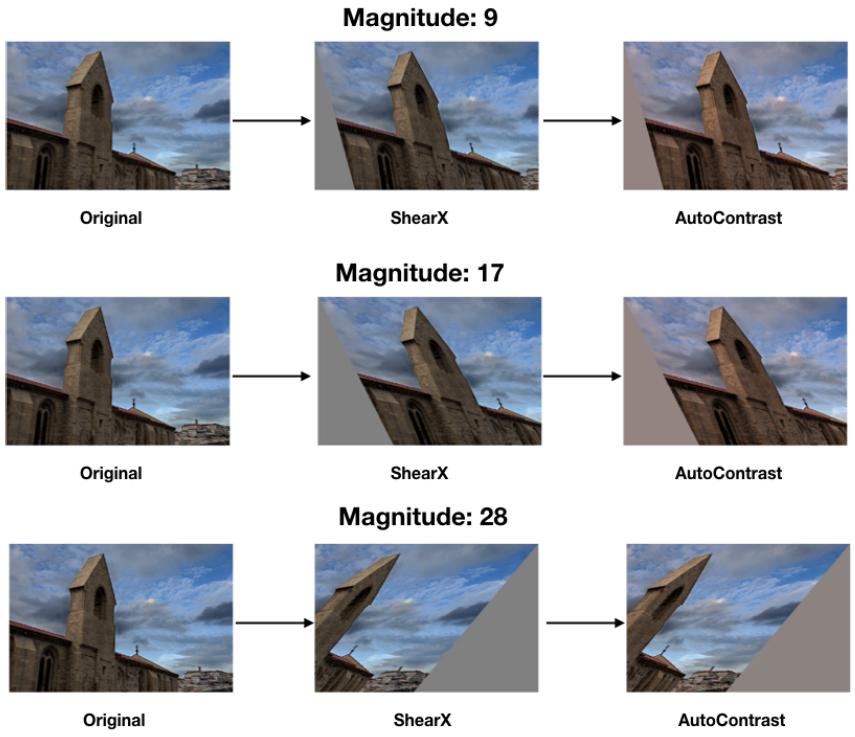
\includegraphics[width=0.6\textwidth]{img/examples}
\caption{N=2 and three magnitudes are shown corresponding to the optimal distortion magnitudes for ResNet-50, EfficientNet-B5 and EfficientNet-B7.}
\end{figure}

\end{frame}
%--------- END Frame 12 -------------
\begin{frame}{RandAugment: justification}

\textbf{Is this going to be better than AutoAugment?}

\begin{itemize}
\item obviously faster than running 15000 trainings on proxy task
\item results from proxy task do not translate that well to the real task
\item both of these change optimal augmentation:
\begin{itemize}
\item dataset size
\item model size
\end{itemize}

\end{itemize}

\end{frame}
%--------- END Frame 12 -------------
\begin{frame}{Model and dataset size affect best magnitude}
\begin{figure}[h]
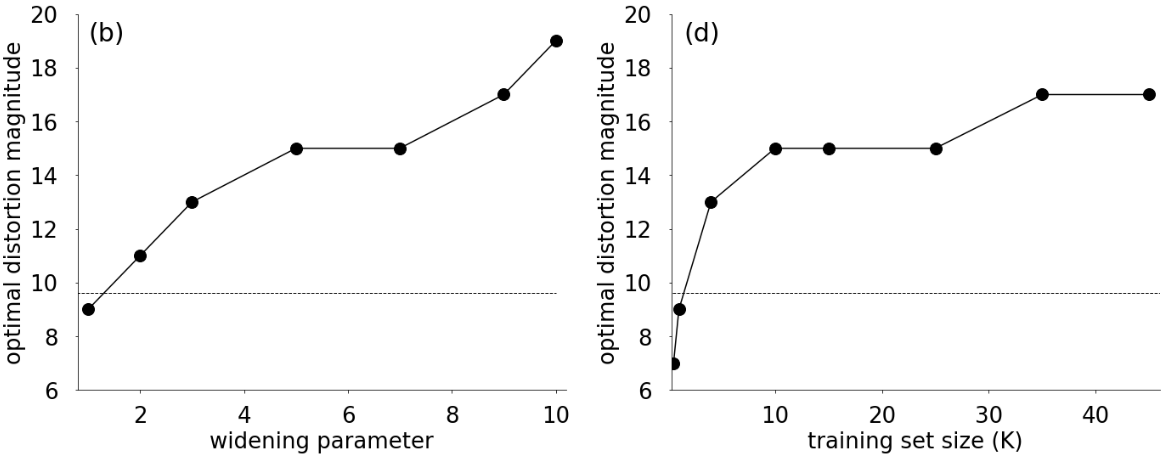
\includegraphics[width=\textwidth]{img/proxy}
\caption{Uses CIFAR-10 validation accuracy for Wide-ResNet architectures averaged over 20 random initializations, N = 1. Dashed line = properly scaled M found by AutoAugment on proxy task.}
\end{figure}
\end{frame}
%--------- END Frame 12 -------------
\begin{frame}{Results: ImageNet}
\begin{figure}[h]
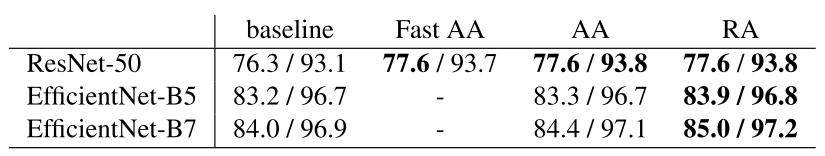
\includegraphics[width=\textwidth]{img/imagenet}
\caption{Top-1 and Top-5 accuracies (\%) on ImageNet. Baseline,  AutoAugment (AA), Fast AutoAugment (Fast AA) taken from sources (see paper).}
\end{figure}
\end{frame}
%--------- END Frame 12 -------------
\begin{frame}{Results: COCO detection task}
\begin{figure}[h]
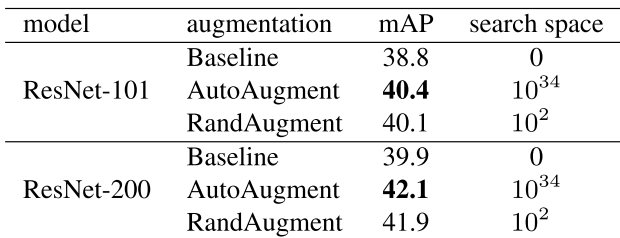
\includegraphics[width=0.8\textwidth]{img/coco}
\caption{Models are trained for 300 epochs from random initialization. AutoAugment used extra transformations to augment the localized bounding box. AutoAugment used 15K GPU hours, where as RandAugment was tuned on 6 values.}
\end{figure}
\end{frame}
%--------- END Frame 12 -------------
\begin{frame}{Results: CIFAR, SVHN}
\begin{figure}[h]
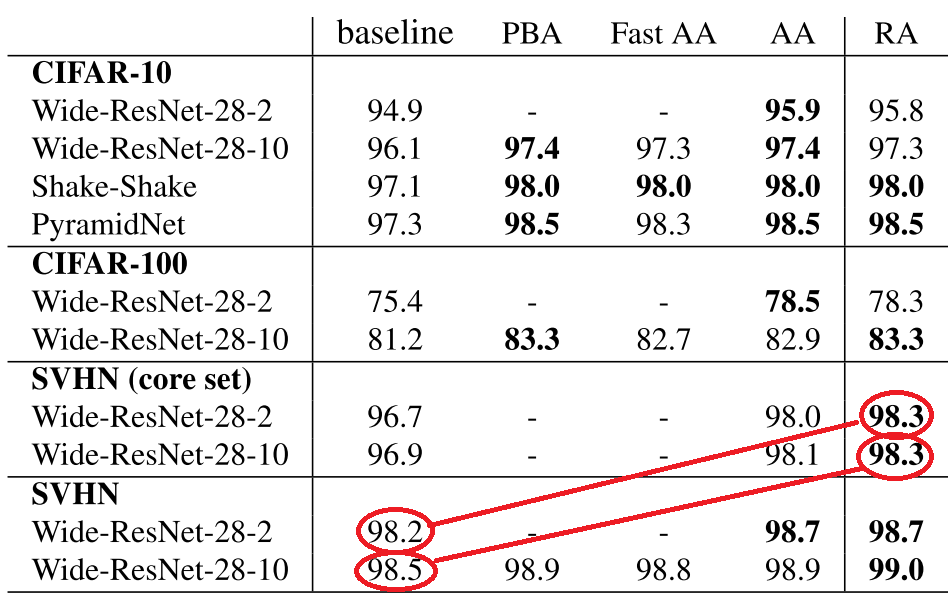
\includegraphics[width=0.8\textwidth]{img/svhn}
\caption{Test accuracy (\%). AA, RA results averaged over 10 independent runs. SVHN core set consists of 73K examples. Full SVHN has extra 531K easier examples to help training but RA has same acc.}
\end{figure}
\end{frame}
%--------- END Frame 12 -------------
\begin{frame}{Adding possible transformations improves accuracy}
\begin{figure}[h]
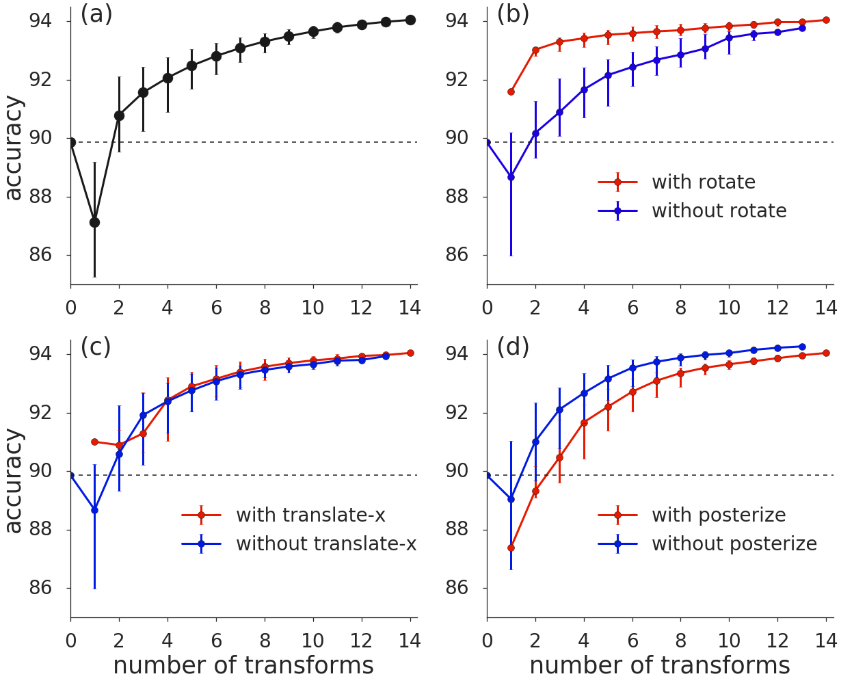
\includegraphics[width=0.6\textwidth]{img/N}
\caption{Median CIFAR-10 validation accuracy for Wide-ResNet-28-2 model architectures trained with RandAugment (N = 3, M = 4) using randomly sampled subsets of transformations. No other data augmentation is included in training. Dashed line = no augmentations. Posterize hurts accuracy.}
\end{figure}
\end{frame}
%--------- END Frame 12 -------------
\begin{frame}{Individual effects of transformations}
\begin{figure}[h]
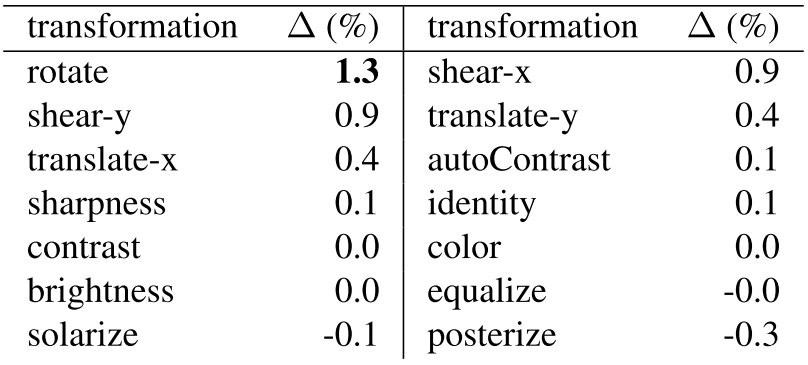
\includegraphics[width=0.8\textwidth]{img/trans}
\caption{Average improvement due to each transformation. Average difference in validation accuracy (\%) when a particular transformation is added to a randomly sampled set of transformations. Wide-ResNet-28-2 trained on CIFAR-10 using RandAugment (N = 3, M = 4) with the randomly sampled set of transformations, with no other data augmentation.}
\end{figure}
\end{frame}
%--------- END Frame 12 -------------
\begin{frame}{Conclusion}

\textbf{Main}:
\begin{itemize}
\item slightly better accuracy for 2 hyperparams, try: 
\begin{itemize}
\item $N \in \{1, 2, 3\}$
\item $M \in \{6, 12, 18, 24\}$ on uniform scale $1$ - $30$

\end{itemize}

\item try stronger augmentation when enlarging datasets and models
\end{itemize}

\vfill

\textbf{Other}:
\begin{itemize}
\item linearly increasing magnitude during training does not help = magnitude = M = constant during training
\item SOTA +1.0\% on ImageNet when used on EfficientNet-B7 
\end{itemize}

\end{frame}

%--------- END Frame 12 -------------
\begin{frame}{Sources}
\begin{thebibliography}{0}

  \bibitem[1]{cit:paper} 1. Cubuk, Ekin D., et al. "Randaugment: Practical automated data augmentation with a reduced search space." Proceedings of the IEEE/CVF Conference on Computer Vision and Pattern Recognition Workshops. 2020. \url{https://arxiv.org/abs/1909.13719} 
  
   \bibitem[2]{cit:auto} 2. Cubuk, Ekin D., et al. "Autoaugment: Learning augmentation policies from data." arXiv preprint arXiv:1805.09501 (2018). \url{https://arxiv.org/abs/1805.09501} 
   
\end{thebibliography}
\end{frame} 
\end{document}
